\documentclass[a4paper]{article}
%\documentclass[varwidth=true, crop=true, border={30pt 10pt}, convert={command=\unexpanded{pdftocairo -r 600 -png \infile\space}}]{standalone}
%\documentclass[tikz, convert, convert={command=\unexpanded{pdftocairo -r 600 -png \infile\space}}]{standalone}
%\usepackage{ctex}
%\usepackage[scheme=chinese, heading=true]{ctex}
%\usepackage{showframe}
%\usepackage{layout}
\usepackage[left=2.5cm, right=2.5cm,top=1.5cm, bottom=1.5cm]{geometry}
\usepackage[heading = true]{ctex}
\usepackage{calc}
\usepackage{graphicx}
\usepackage{enumitem}
%\usepackage{xeCJK}
%\setCJKmainfont{FangSong_GB2312}
%\setCJKmainfont{FandolSong}
%\setCJKmainfont{Microsoft YaHei}
%\setCJKmainfont{Microsoft YaHei Light}
\setCJKmainfont{Source Han Serif SC}[%
UprightFont     = * SemiBold,
BoldFont        = * Heavy,
ItalicFont      = * SemiBold,
BoldItalicFont  = * SemiBold,
RawFeature      = +fwid]
\setCJKmonofont{Sarasa Mono SC}

%\newlength\mylen
%\settowidth\mylen{\medspace}
%\the\mylen
% 1、标题字体常设为二号方正小标宋,如有副标题,可用楷体。
% 2、正文的文件字体用三号仿宋GB2312。
% 3、正文中一级标题用黑体,二级标题用楷体,三级和四级和正文用一样3号仿宋。
% 4、文档层次结构依次可用“一”“(一)”“1.”“(1)”。
\ctexset {
autoindent=true,
figurename=图,
tablename=表,
appendixname=附录,
% part/pagestyle = empty,
% chapter = {
% format = \raggedright,
% pagestyle = empty,
% },
section = {
%	name = {第,条},
	name = {,、},
	%nameformat=\Large\bf,
	indent = 0pt,
%	aftername = \hspace{0.5em}\medskip,
	aftername = \hspace{0pt},
	number = \chinese{section},
	%number = \arabic{section},
	format = \bf\zihao{3},
	%break = \Needspace{.5\textheight},
},
subsection = {
	name = {(,)},
%	indent = 0.2222em,
	indent = 0.55em,
	% nameformat= \Large\bf,
%	aftername = \medspace,
	aftername = \hspace{0pt},
	number = \chinese{subsection},
	%number = \arabic{section},
	format = \bf\zihao{3},
},
% subsubsection = {
% name = {,.},
% % nameformat= \Large\bf,
% aftername = \space,
% number = \arabic{subsubsection},
% %number = \arabic{section},
% format = \zihao{3},
% nameformat = \bigskip\hfill,
% %beforeskip = 12pt,
% },
%paragraph = {
% name = {,.},
% % nameformat= \Large\bf,
% aftername = \space,
% %number = \arabic{subsubsection},
% %number = \arabic{section},
% format = \zihao{3},
% nameformat = \bigskip\hfill,
%beforeskip = 20pt,
%afterskip = 20pt,
%},
}

\setlist[enumerate,1]{
%	label = \bf\arabic*.,
	labelwidth = 1em,
	itemindent = 3em,
	leftmargin = 0em,
	listparindent = 2em,
%	labelsep= 0pt	
}
\setlist[enumerate,2]{
%	label = \bf\arabic*.,
	label = (\bf\arabic*),
	labelwidth = 1em,
	itemindent = 5em,
	leftmargin = 0em,
	listparindent = 2em,
%	labelsep= 0pt	
}
\title{%
%\vspace{-4ex}
\zihao{2}\textbf{成本费用分析报告编制方法}%
%\vspace{-9ex}
}
\author{}
\date{}
\begin{document}
%	\layout
\maketitle
\pagestyle{plain}
%\newlength\mylen
%\settowidth\mylen{\medspace}
%\the\mylen
\zihao{3}
%\renewcommand\normalsize{\fontsize{16}{20.8}\selectfont}
%\normalsize
很多企业都很重视开源节流,但往往对费用分析不够重视,节流针对性不强,或者不知道如何分析,拔剑四顾心茫然。对于企业而言,财务做好分析等于给企业做了一个诊断,往往通过费用分析可发现一些问题,从而未雨绸缪。

每个财务人员都会遇到被老板要求提供费用分析报告的时候。
如何呈现出一份完美的费用分析报告,这是每个财务人员必须要掌握的技能。
下面就带你一步步Get这个技能!


\section{切忌胡子眉毛一把抓}

一个企业主要分析的对象有:

\subsection{人力成本分析}

人是企业产生效益的主要资源,用人成本也是企业关心的。主要侧重于人工效率分析,如何提高人工效率,为企业创造更大效益。

\subsection{主营成本分析}

主营成本是企业经营的主要成本,也是分析的重点。主要侧重于成本利润率分析,如何降低成本利润率。

\subsection{专项费用}

今年新增加的专项费用,比如本期立项的工程、本期开展的活动、本期新产品的研发费用。专项费用分析主要侧重于“投入—产出”的分析,企业对新增费用比较关注投入能带来的收益,或者投资的回报。

\subsection{其他波动较大费用分析}

分析原因,提出解决方案。

所有事后结果分析,剖析原因的目的是为了更好的发现根本问题,对已经发生事情进行总结反思,所以解决问题的根本点一定是在事前。做费用分析的目的也一定是为了更好的为企业的决策服务。

\section{用财务数据说话}

首先进行总体分析,总体分析是做数据趋势的判断,主要方式:

\subsection{单一数据的同期比、预算比、或者几年数据的趋势分析;}
\subsection{费用使用效率指标的同期比、预算比等;}
单一数据的对比分析让我们对费用的整体情况有个把握,但不管是增加还是降低,每个数据波动都是一个疑问,带着这个疑问结合指标分析,判断重点分析对象。

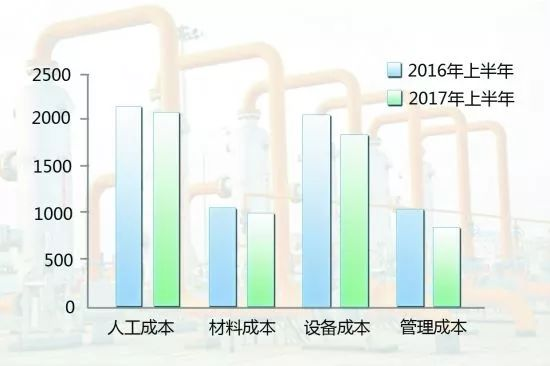
\includegraphics[width=0.8\textwidth]{./figure/cost_diagram.jpeg}
\subsection{指标分析}
\begin{enumerate}
	\item 成本率
	
	成本率指标的计算,为了识别成本费用结构波动。不管异常出现在哪个方向,主营业务成本和人工费用必须进行剖析,如果有异常则带着疑问去剖析,如果没有异常则带着“能否更好”的心态去剖析。所以总体指标分析,仅仅分析的是趋势,让我们知道问题点,从而带着问题去做明细分析。
	
	\item 人工指标
	
	人工效率指标一般包括人均收入贡献、人均利润贡献、人均工资、每元工资带来的收入等。\\	
	人工效率指标表示公司对人的投入能带来的产出,我们的目标是合理减少投入增加产出;对这一指标的计算帮助我们看出本年度的人工效率趋势,便于识别问题点进行明细分析。
	
	\item 其他成本指标
	
	材料使用效率指标:单位产品直接材料、单位产品物料消耗、单位产品能源消耗(单位面积能源消耗、日均能耗)、材料损耗率等。
	
	物品使用效率指标:固定资产周转率、单位宣传费带来的收入、人均办公用品、单位面积维修费等。	
	对成本使用效率指标的计算帮助我们判断成本费用趋势,发现问题点,在明细分析阶段剖析问题,提出解决方案。
	
	
\end{enumerate}

对成本使用效率指标的计算帮助我们判断成本费用趋势,发现问题点,在明细分析阶段剖析问题,提出解决方案。

\subsection{期间费用分析}
期间费用每个企业基本相同,期间费用主要的分析方法:

\begin{enumerate}
	\item 销售费用
	
	评价销售业绩,主要用“投入—产出”分析,如活动费、广告费、销售佣金,付出的费用有没有产生目标效益。
	\item 管理费用
	
	评价管理效率,主要对预算对比和同期对比波动大额的费用进行明细分析。
	
	\item 财务费用
	
	评价资金管理成效,主要针对公司业务的特殊性,对pos手续费、汇兑损益和利息支出等进行明细分析。

	\item 人工分析
	
	评价人工效率,各期间费用中涉及人工成本单独作为分析对象,需要人事部门的专业数据分析。
%以下内容为测试四级标题格式
%	\begin{enumerate}
%		\item 中文广州
%		
%		人工效率指标一般包括人均收入贡献、人均利润贡献、人均工资、每元工资带来的收入等。	
%		人工效率指标表示公司对人的投入能带来的产出,我们的目标是合理减少投入增加产出;对这一指标的计算帮助我们看出本年度的人工效率趋势,便于识别问题点进行明细分析。
%		
%		\item 中文广州
%		
%		人工效率指标一般包括人均收入贡献、人均利润贡献、人均工资、每元工资带来的收入等。	
%		人工效率指标表示公司对人的投入能带来的产出,我们的目标是合理减少投入增加产出;对这一指标的计算帮助我们看出本年度的人工效率趋势,便于识别问题点进行明细分析。
%		
%		\item 中文广州
%		
%		人工效率指标一般包括人均收入贡献、人均利润贡献、人均工资、每元工资带来的收入等。	
%		人工效率指标表示公司对人的投入能带来的产出,我们的目标是合理减少投入增加产出;对这一指标的计算帮助我们看出本年度的人工效率趋势,便于识别问题点进行明细分析。
%	
%	\end{enumerate}	

\end{enumerate}

\section{编写一份完美的费用分析报告}

\subsection{抛出分析的结论,吸引被报告者的眼球}
	
对于分析类的报告,使用者往往最先关注的是分析得出的结论,抓住分析的结论就抓住了报告使用者的眼球。

\subsection{用数据对结论加以支持}

任何财务分析都是在准确无误的数据支持下完成的,只有具备足够的数据支持才能使分析的结论让人信服。

\subsection{提出建议对策}
%\begin{enumerate}[label=({\arabic*})]
%	\item aa
%	\item bb
%	\item cc
%\end{enumerate}
好的财务分析是为企业服务的,没有解决方案的分析等于没有分析,所以财务分析最具有实践意义的部分就是以专业的角度对分析的问题提出解决的对策。

\end{document}
